% !TEX root = /home/eb/.vscode/extensions/qftrules.programme-colle/tmp/Exercice.tex
\graphicspath{{\pathtoexos/Info/Figures/}}
%%%%%%%%%%%%%%%%%%%%%%%%%%%%%%%%%%%
\begin{exo}[PC][1][devoir]{Étude de graphes}

\subsection{Graphes planaires}
  
\begin{fig}
\centering

\includegraphics[width=0.8\textwidth]{graphes_planaires.png}
%\caption{}
% \label{fig:}
\end{fig}
%%%%%%%%%%%%%

Tous les graphes considérés sont non orientés et sans boucle.
\begin{quest}
\item Donner la définition formelle de graphe non orienté.
\sol{
 Une graphe non orienté $G$ est un couple $G = (S, A)$ où $S$ est un ensemble fini et :
$A \subset \{ \{x, y\} : (x, y) \in S^2 \}.$
$S$ s’appelle l’ensemble des sommets et $A$ s’appelle l’ensemble des arêtes.

}
\item Donner la définition de boucle.
\sol{
Une boucle est une arête de la forme $\{s, s\}$ où $s \in S$.

}
\end{quest}
Dans tout le sujet, les sommets d’un graphe $G$ avec $n$ sommets sont systématiquement étiquetés par $0, 1, 2, . . . , n - 1$; chaque entier $i \in \{0,1,...,n - 1\}$ est donc l’étiquette d’un et un seul sommet de $G$.


En \texttt{python}, un graphe est représenté par une liste \texttt{G: list[list[int]]} telle que \texttt{G[i]} est la liste d’adjacence
du sommet d’étiquette $i$ (cette liste ne contient jamais d’élément en double). Par exemple, le graphe de la \textsc{Figure}
1 correspond à :
\begin{center}
\texttt{G\lstinline{_}fig1 = [[2,3,4], [2,3,4], [0,1,3,5], [0,1,2,4,5], [0,1,3], [2,3]].}%\lstinline{}
\end{center}

\begin{quest}
\item Donner les listes \texttt{G\_fig2} et \texttt{G\_fig3} pour représenter les graphes des \textsc{Figures} 2 et 3.
\sol{
Les listes sont identiques :

\begin{center}
\texttt{G\_fig3 = [[1 ,2 ,3 ,4] , [0 ,2 ,3 ,4] , [0 ,1 ,3 ,4] , [0 ,1 ,2] , [0 ,1 ,2]]}
\end{center}

}
\end{quest}

Dans la suite, le type \texttt{list[list[int]]} sera noté \texttt{graphe}. Ainsi une fonction \texttt{f(G: graphe) -> int} est
une fonction qui prend en entrée un graphe représenté par une liste \texttt{G} de type \texttt{list[list[int]]}, et qui renvoie
un entier.


\fbox{
\parbox{0.97\textwidth}{
\textbf{Définition 1}. Un graphe $G$ est dit \emph{planaire} s’il peut être être dessiné dans le plan sans que deux
arêtes ne se croisent.
}
}


Par exemple, le graphe de la \textsc{figure} 1 est planaire alors que le graphe de la \textsc{figure} 4 n’est pas planaire. De
plus, contrairement aux apparences, le graphe de la \textsc{figure} 2 est planaire. En effet, les \textsc{figures} 2 et 3 représentent
le même graphe. Puisque le graphe de la \textsc{figure} 3 est planaire, le graphe de la \textsc{figure} 2 l’est aussi.

\begin{quest}
\item Montrer par un dessin que le graphe de la \textsc{figure} 5 est planaire.
\sol{
On dessine le graphe sans que les arêtes ne se croisent
% \begin{center}
  \begin{fig}
    \centering
    % 
\includegraphics[width=0.8\textwidth]{graphes_planaires.png}
    %\caption{}
    % \label{fig:}
    
\includegraphics[scale=0.3]{graphe5.png}
  \end{fig}
  % \end{center}
  }
\end{quest}

\subsection{Graphes complets}

\fbox{
\parbox{0.97\linewidth}{
\textbf{Définition 2}. Un graphe $G$ est dit \emph{complet} si tous les sommets sont adjacents deux à deux, c'est-à-dire que tout couple de sommets disjoints est relié par une arête.
}
}

\begin{quest}
\item On note $K_n$ le graphe complet à $n$ sommets. Représenter $K_3$ et $K_4$.
\item Écrire une fonction \texttt{make\_complet} qui renvoie le graphe complet à $n$ sommets, et vérifie les spécifications suivantes.
\inputminted{python}{\pathtoexos/Info/Scripts/make_complet.py}
\sol{
  \rm
\inputminted{python}{\pathtoexos/Info/Scripts/make_complet_sol.py}
}
\item Exécuter l'algorithme ci-dessus pas à pas sur le cas $n=4$.
\end{quest}
On rappelle que les graphes considérés dans ce sujet sont sans boucle et que les listes d’adjacence ne
contiennent pas d’élément en double.
\begin{quest}
\item Quelle propriété possède la longueur des lignes de la liste d’adjacence d’un graphe complet d'ordre $n$ ?
\sol{
Longueur $n-1$.
}
\item Écrire une fonction \texttt{est\_complet} qui indique si le graphe donné en entrée est complet avec $n$ sommets, et vérifie les spécifications suivantes. Votre fonction devra être de complexité $O(n)$. On expliquera
rapidement le choix d’implémentation.
\inputminted{python}{\pathtoexos/Info/Scripts/est_complet.py}
\sol{
\inputminted{python}{\pathtoexos/Info/Scripts/est_complet_sol.py}
}
\item Montrer que votre fonction est bien de complexité $O(n)$.
\sol{
Toutes les opérations utilisées dans la fonction \texttt{est\_complet} sont élémentaires et s’exécutent
en temps constant. Il y a une boucle for qui exécute au plus n tours de boucle.
En conclusion, le temps d’exécution est bien en $O(n)$.

}
\end{quest}

\end{exo}
%%%%%%%%%%%%%%%%%%%%%%%%%%%%%%%%%%%


%%%%%%%%%%%%%%%%%%%%%%%%%%%%%%%%%%%
\begin{exo}[PC][1][TD]{Stratégies au jeu de Nim}

Nous étudions dans tout cet exercice le jeu de Nim $(n=5,p=2)$. 
% La \Sec{impl} présente l'implémentation du graphe du jeu sous forme de dictionnaire.
    % On considère un jeu de Nim avec un tas d’objets où chaque joueur peut retirer de $1$ à $p$ objets. Celui que ne peut plus retirer d'objets a perdu. Une position est déterminée par le nombre $i>0$ d'objets présents dans le tas. On note $n$ le nombre d’objets initial.

\parag{Implémentation du jeu}
\label{sec:impl}
On commence par implémenter le graphe du jeu sous forme de dictionnaire.

\begin{quest}
\item Représenter graphiquement un graphe orienté \emph{simple} $G_s$ associé au jeu de Nim $(n=5,p=2)$. Définir formellement le graphe $G_s=(S,A)$, ainsi que l'origine $s_0$ et les sommets finaux $F$.

\sol{
Voir cours. Le graphe orienté $G_s=(S,A)$ est la donnée d'un ensemble de sommets $S$ et d'arcs $A$. 
\begin{enumerate}
  \item 
  En nommant le sommet $i$ par le nombre d'objets restants, on a au plus simple,
  \eqbox{
    S=\{5,4,3,2,1,0\}, 
    }
    qui comprend $m=6$ éléments. 
    
    \item L'ensemble des arcs $A$ est donné par
    \eqbox{
      A=\{(4,3),(4,2),(3,2),(3,1),(2,1),(2,0),(1,0)\}.
      }
    \item Le sommet initial (origine) est 
      \eqbox{
        s_0=5.
        }
    \item L'ensemble des sommets finaux est 
        \eqbox{
          F=\{0\}.
          }
  \end{enumerate}
}
\sol{
Le graphe peut se représenter de la manière suivante.
\begin{fig}[label]
  \centering
  
\includegraphics[scale=1]{nim_simple}
  %\capt{}
\end{fig}
}

\item Rappeler les définitions d'une matrice d'adjacence et d'une liste d'adjacence. Donner la matrice d'adjacence et la liste d'adjacence du graphe $G_s$ défini précédemment. Quelle est la complexité $C(n,p)$ pour implémenter la liste d'adjacence du graphe simple d'un jeu de Nim $(n,p)$ ?
\sol{
  \udl{Matrice d’adjacence} :
  \begin{center}
    matrice carrée $M \in \mc{M}_m(\{0,1\})$, où $m=card(S)$ est l'ordre du graphe, dont les entrées vérifient
    \eqbox{
      M_{ij} = \begin{cases}
        1 & \text{si } (i,j) \in \mc{A} \\
        0 & \text{sinon}.
      \end{cases}
      }
      
    \end{center}
    Autrement dit, l’élément $M_{ij}$ vaut $1$ si le sommet $j$ est un successeur du sommet $i$, et $0$ sinon. La matrice a autant de lignes et de colonnes que de sommets du graphe.
  Pour le graphe simple $G$ défini précédemment, la matrice d’adjacence est :
  % \[
  \eqbox{
    M = \begin{pmatrix}
      0 & 0 & 0 & 0 & 0 & 0 \\
      1 & 0 & 0 & 0 & 0 & 0 \\
      1 & 1 & 0 & 0 & 0 & 0 \\
      0 & 1 & 1 & 0 & 0 & 0 \\
      0 & 0 & 1 & 1 & 0 & 0 \\
      0 & 0 & 0 & 1 & 1 & 0 \\
    \end{pmatrix}.
    }
    % \]
    \udl{Remarque}.
    \begin{itemize}
      \item 
      La ligne $i=0$ remplie entièrement de zéro (sans successeurs) correspond aux sommets finaux. 
      \item La colonne $j=5$ remplie entièrement de zéro (sans antécédents) correspond à l'origine. 
    \end{itemize}
}
\sol{
  \udl{Liste d’adjacence} : 
  \begin{center}
    liste $L$ de listes $L_i, i\in\{0,\ldots,m-1\}$, vérifiant 
    \eqbox{
      L_i = \{ j \in \{0,\ldots,m-1\} : (i,j) \in \mc{A} \}.
    }
  \end{center}
Autrement dit, $L$ est la liste des listes $L_i$ des successeurs de chaque sommet $i$.
  Pour le graphe simple $G_s$ défini précédemment, la liste d’adjacence est :
  % \[
  \eqbox{
    L = [\,[~], [0], [0,1], [1,2], [2,3], [3,4]\,].
    }
  % \]
  Déterminons la complexité $C(n, p)$ pour implémenter la liste d’adjacence du jeu de Nim $(n,p)$. 
  
  
  Il faut définir pour cela :
  \begin{itemize}
    \item 
    une liste de $p$ successeurs pour chacun des $n+1-p$ sommets non antécédents du sommet final ;
    \item les listes de $1+\ldots+(p-1) = \frac{p(p-1)}{2}$ successeurs pour les $p$ sommets antécédents du sommet final. 
  \end{itemize}
  On a donc
  \eqbox{
    C(n, p) = p\left(n+1-\frac{p+1}{2} \right) = O(mp),
  }
  où $m = n+1$ est l’ordre du graphe.
  On peut comparer à la complexité de la matrice d’adjacence, qui est $O(m^2)$. Pour $p$ petit devant $m$, il est donc moins coûteux d’implémenter la liste d’adjacence.
}

\item Représenter graphiquement un graphe orienté \emph{biparti} $G$ associé au jeu de Nim $(n=5,p=2)$. Chaque sommet est de la forme $s=(i,j)$, où $0\leq i\leq n$ représente le nombre d'objets, et $j=1$ ou $2$ le joueur. Implémenter ce graphe en \texttt{python} sous forme d'un dictionnaire \texttt{G}, où chaque clé est un sommet \texttt{(i,j)} et chaque valeur \texttt{G[(i,j)]} représente la liste des successeurs de \texttt{(i,j)}.
 % sur votre feuille.

 \sol{
  On peut représenter le graphe orienté biparti $G$ sous la forme de deux colonnes reliées par des arcs. Chaque colonne correspond à un ensemble $S_1$ ou $S_2$ de sommets appartenant aux joueurs $j=1$ ou $j=2$.
 \begin{fig}[label]
  \centering
  
\includegraphics[scale=1]{nim_biparti}
  %\capt{}
 \end{fig}
 }
 \sol{
 On peut implémenter $G$ sous forme d'une liste d'adjacence en utilisant la classe \texttt{dict} (dictionnaire) de \texttt{python}.
 \inputminted[linenos=false,frame=single]{python}{\pathtoexos/Info/Scripts/G.py}
 
 }
% \sol{


% % Graphe biparti $G=(S,A)$ : ensemble de sommets $S=\{(1,5),(2,4),(2,3),(1,3),(1,2),(1,1),(2,2),(2,1)\}$
% % comprenant $m=8$ éléments, sommet initial $s_0=(1,5)$, ensemble des arcs $A=\{((1,5),(2,4)),((1,5),(2,3)),((2,4),(1,3)),((2,4),(1,2)),((2,3),(1,2)),((2,3),(1,1))\}$. Les sommet finaux sont $F=\{2,1\}$.
% }

% \item  Que vaut la complexité $C(n,p)$ lorsqu’on implémente le graphe d’un jeu de cette façon ?
% Définir à la main, puis sur \texttt{python}, un graphe $G$ dont chaque clé représente un sommet et est constitué d'une paire $(j,n)$ où $j$ est le joueur qui contrôle le sommet et $n$ le nombre d'objets restant, et chaque valeur représente la liste des sommets successeurs.
% \sol{
% La matrice d’adjacence est une matrice $M$ de taille $m\times m$ où $m$ est le nombre de sommets. L’élément $M_{ij}$ vaut $1$ si le sommet $j$ est un successeur du sommet $i$, et $0$ sinon. La liste d’adjacence est une liste $L$ de taille $m$ où chaque élément $L_i$ est une liste des successeurs du sommet $i$.

% \inputminted[linenos=true]{python}{\pathtoexos/Info/Scripts/G.py}

% Si $m = \text{card}(S)$ désigne l’ordre du graphe (nombre de sommets) et $a=\text{card}(A)$ le nombre d’arcs, alors $C=O(m+a)$. Ici le nombre de sommets vaut $s = 2(n-1)$ (pour $n>p+1$) et le nombre d’arcs vaut environ $a = p\times 2(n-p)$, soit $C(n,p) = O(2(p+1)n)-2(1+p^2)) = O(2(p+1)n)$ à $p$ fixé lorsque $n$ est grand.
% }
\item En pratique, il est fastidieux de définir manuellement le graphe biparti associé au jeu de Nim pour les grandes valeurs de $n$. On propose donc de définir une fonction récursive \texttt{nim}  qui construit le graphe orienté biparti associé au jeu de Nim $(n,p=2)$. Commenter et compléter le code ci-dessous.
Effectuer l'exécution pas à pas de l'appel \texttt{G=\{\};nim(G,5,1)}. Exécuter ce code sur \texttt{python} puis vérifier que la variable \texttt{G} correspond bien au graphe orienté biparti du jeu de Nim $(n=5,p=2)$.
\inputminted[linenos=true,frame = single]{python}{\pathtoexos/Info/Scripts/nim_trou.py}
% Écrire la fonction récursive \texttt{nim}, qui prend en argument un entier $n$ (nombre d'objets), un entier $j$ (numéro du joueur), et un dictionnaire $G$ (le graphe du jeu).
\sol{
% Cette fonction crée le graphe orienté biparti $G$ associé à un jeu de nim $(n,p=2)$.
\rm{
\inputminted[linenos=true,frame = single]{python}{\pathtoexos/Info/Scripts/nim_trou_sol.py}
}
}
\sol{
On peut effectuer l'exécution pas à pas en suivant à chaque appel de la fonction récursive la valeur des variables locales \texttt{n}, \texttt{j}, \texttt{adv}, \texttt{G[(n,j)]}, ainsi que laquelle des conditions \texttt{n >= 2}, \texttt{n == 1} ou \texttt{n == 0} est vérifiée. On peut également indiquer le dictionnaire complet \texttt{G} si la place le permet. La représentation sous forme de tableau est adaptée. Il est nécessaire d'initialiser \texttt{G} au dictionnaire vide avant le premier appel de la fonction \texttt{nim}.
\rm{
\begin{center}
\newcommand\tikzmark[2]{%
\tikz[remember picture] \node[inner sep=2pt,outer sep=0] (#1){#2};%
}

\newcommand\link[4]{%
\begin{tikzpicture}[remember picture, overlay, >=stealth, shift={(0,0)}]
  \draw[->,>=latex] (#1)  ++ (#4,0) -- ++ (-#3,0) -- ++ (0,#2) -- ++ (#3,0);
\end{tikzpicture}%
}

\begin{tabular}{|c|c|c|c|c|c|}
\hline
\texttt{n} & \texttt{j} & \texttt{adv} & condition & \texttt{G[(n,j)]}  \\
\hline
\tikzmark{a}{5} & 1 & 2 & \texttt{n>=2} & \texttt{[(4,2),(3,2)]} \\
\hline 
4 & 2 & 1 & \texttt{n>=2} & \texttt{[(3,1),(2,1)]}\tikzmark{b}{} \\
\hline
\tikzmark{c}{3} & 1 & 2 & \texttt{n>=2} & \texttt{[(2,2),(1,2)]} \\
\hline
2 & 2 & 1 & \texttt{n>=2} & \texttt{[(0,1),(1,1)]}\tikzmark{d}{}  \\
\hline
\tikzmark{e}{1} & 1 & 2 & \texttt{n==1} & \texttt{[(0,2)]} \\
\hline
0 & 2 & 1 & \texttt{n==0} & \texttt{[]} \\
\hline
\dots & \dots & \dots & \dots & \dots \\
% 0 & 1 & 2 & \texttt{n==0} & \texttt{[]} \\
% \hline
% 1 & 2 & 1 & \texttt{n==1} & \texttt{[(0,1)]}\tikzmark{f}{} \\
% \hline
% \tikzmark{g}{2} & 1 & 2 & \texttt{n>=2} & \texttt{[(0,2),(1,2)]} \\
% \hline
% 3\tikzmark{h}{}  & 2 & 1 & \texttt{n>=2} & \texttt{[(2,1),(1,1)]} \\
% \hline
\hline
\end{tabular}
% \link{a}{-0.55}{2}{-0.5}
% \link{b}{-0.5}{-1.5}{0.4}
% \link{c}{-0.5}{1}{-0.5}
% \link{d}{-0.45}{-0.5}{0.4}
% \link{e}{-0.55}{0.5}{-0.5}
% \link{d}{-1.2}{-0.5}{0.4}
% \link{c}{-2.2}{1}{-0.5}
\end{center} 
On représente ci-dessus uniquement la première pile d'exécution, qui mène au sommet final $(0,2)$. Il faut ensuite remonter la pile d'exécution en complétant les autres appels récursifs. On remarque que cet algorithme n'est pas optimal, puisqu'il repasse plusieurs fois par les mêmes sommets. Nour verrons plus loin comment optimiser le parcours pour l'algorithme min-max.
}
}
% \item Représenter le graphe du jeu et identifier toutes les stratégies gagnantes pour le premier joueur sur l'arbre de décision correspondant.
\item \textsc{Bonus} : généraliser la fonction \texttt{nim} à une valeur de $p$ quelconque. Utiliser cette fonction pour générer le graphe représentatif du jeu de nim $(n=9,p=3)$.
\sol{
  On peut pour cela essayer d'ajouter itérativement les successeurs possibles de \texttt{(n,j)} en utilisant une boucle \texttt{while},tout en appelant récursivement la fonction \texttt{nim} pour chaque successeur ajouté.
  \rm{
  \inputminted[linenos=true,frame=single]{python}{\pathtoexos/Info/Scripts/nim_p_sol.py}
}}
\end{quest}


\parag{Nombre de Grundy} On se propose de déterminer les stratégies gagnantes du jeu de Nim à partir d’un théorème mathématique appelé théorème de Sprague-Grundy.
  À chaque sommet $(i,j)$ appartenant au joueur $j$ contenant $i$ objets, on associe le nombre noté $g(i)$, appelé nombre de Grundy, défini par :
  $$
  \left\{
  \begin{array}{l}
  g(i)=i \text{ si $1\leq i\leq p$ (sommet final)},\\
  g(i)=\min \{ \N \backslash \{g(i-\ell), \forall \ell \in \llbracket 1,p \rrbracket \} \} \text{ sinon}.
  \end{array}
  \right.
  $$
  % \begin{liste}
  %   \item le nombre de Grundy de la position où tous les objets sont retirés vaut $0$, soit $g(0)=0$ ;
  %   \item le nombre de Grundy d'une position $i>0$ est le plus petit entier naturel qui n'est pas le nombre de Grundy d'une des positions directement atteignables depuis la position $i$.
  % \end{liste}
L'ensemble $\{g(i-\ell), \forall \ell \in \llbracket 1,p \rrbracket \} $ représente l'ensemble des nombres de Grundy des successeurs de $i$.
  On commence par étudier le jeu de Nim pour $p=2$.
  Par exemple, depuis la position $i=4$ on peut atteindre les positions $3$ et $2$. Si $g(3)=0$ et $g(2)=2$, alors $g(4)=\min\{1,3,4,...\}=1$.

  \begin{quest}
    %\item Le nombre de Grundy correspond-il à la définition d'une heuristique ? Justifier.
      \item Montrer par récurrence sur $i$ que $g(i)$ est égal au reste de la division euclidienne de $i$ par $3$, soit 
      \begin{equation}
        \forall i \in \N^*, g(i)=r, \text{ avec } i=3q+r, 0\leq r\leq 2.
      \end{equation}
      \sol{
      \begin{liste}
        \item \udl{Hypothèse}. $H_i$ : $g(i)=r,  \text{ avec } i=3q+r, 0\leq r\leq 2$.
        \item \udl{Initialisation}. Pour $i=1$, nous avons $g(1)=1$ par définition. Or la division euclidienne de $1$ par $3$ donne $1=3\times 0+1$. Donc $H_1$ est vraie.
         %Soit une position $r$ tell que $0\leq r \leq p$. On montre que $g(r) = r$.
          %Depuis la position $0 \leq r \leq p$, un joueur peut atteindre toutes les positions de $0$ à $r-1$, et donc $g(r)=r$.
          \item \udl{Hérédité}. Supposons que $H_i$ est vraie pour tout $i \leq n$. Montrons que $H_{n+1}$ est vraie. Notons $n+1 = 3q+r$ la division euclidienne de $n+1$ par $3$, avec $0 \leq r \leq 2$ et $q\geq1$. Les successeurs de $n+1$ sont $n$ et $n-1$. Étudions les trois cas possibles suivant la valeur du reste $r$.
          \begin{enumerate}
            \item Si $r=0$, alors $n+1=3q$, donc $n-1=3(q-1)+2$ et $n-2=3(q-1)+1$. Les nombres de Grundy des successeurs de $n+1$ valent donc $g(n-1)=2$ et $g(n-2)=1$. Ainsi, $g(n+1) = 0 =r$.
            \item Si $r=1$, alors $n+1=3q+1$, donc $n-1=3q$ et $n-2=3(q-1)+2$. Les nombres de Grundy des successeurs de $n+1$ valent donc $g(n-1)=0$ et $g(n-2)=2$. Ainsi, $g(n+1) = 1 =r$.
            \item Si $r=2$, alors $n+1=3q+2$, donc $n-1=3q+1$ et $n-2=3q$. Les nombres de Grundy des successeurs de $n+1$ valent donc $g(n-1)=1$ et $g(n-2)=0$. Ainsi, $g(n+1) = 2 =r$.
          \end{enumerate}
          On en conclut que $H_{n+1}$ est vraie.
          \item \udl{Conclusion}. Par récurrence, on a montré que 
          \eqbox{
            \forall i \in \N^*, g(i)=r,  \text{ avec } i=3q+r, 0\leq r\leq 2.
          }
      \end{liste}
      }
  \end{quest}
  On admet que ce résultat se généralise à $p$ quelconque :
  \begin{equation}
    \forall i \in \mathbb{N}, g(i)=r,  \text{ avec } i=(p+1)q+r, 0\leq r\leq p.
  \end{equation}
  
  % pour tout entier naturel $i$, le nombre de Grundy vaut $g(i)=r$ où $r$ est le reste de la division euclidienne de $i$ par $p+1$.
    % On pourra raisonner par récurrence sur le quotient $q$ de la division euclidienne $n=q(p+1)+r$.
  \begin{quest}
    \item Le théorème de Sprague-Grundy, établi dans les années 1930, affirme que tout sommet $(i,2) \in S_2$ dont le nombre de Grundy vaut $0$ est une position gagnante pour le joueur $j=1$. En déduire une stratégie gagnante $f$ pour le joueur $j=1$ suivant la valeur de $n$. Existe-t-elle toujours ?
    \sol{
    Le joueur $j=1$ doit atteindre un sommet dont le reste vaut $0$, i.e. qui est un multiple de $p+1$. On peut donc choisir comme stratégie la fonction
    % $$
    \eqbox{
      \begin{array}{rccl}
        f : & S_1 \backslash F & \rightarrow & S_2 \\
        & (i,1)  & \mapsto & (i-r,2) \text{ si } r\geq1,  \\
        & (i,1) & \mapsto & (i-1,2) \text{ si } r=0,
      \end{array}
      }
    % $$
    où $r$ désigne le reste de la division euclidienne de $i$ par $p+1$. La disjonction de cas pour $r=0$ est nécessaire car $((i,1),(i,2))$ n'est pas un arc du graphe.
    Cette stratégie n'est gagnante que si le joueur $j=2$ ne puisse pas atteindre un sommet $(i,2)$ avec $i$ multiple de $p+1$, ce qui est possible ssi $n$ n'est pas un multiple de $p+1$.
    }
    % \item Représenter le graphe du jeu $G$ pour $n=5$ et $p=2$.
    % \sol{
    % \begin{fig}[]
    %   \centering
    %   
\includegraphics[width=0.3\textwidth]{Grundy_jeu.png}
    %   
\includegraphics[width=0.5\textwidth]{Grundy_biparti_jeu.png}
    %   \capt{}
    % \end{fig}
    % }
    % %, où chaque sommet correspond à une position $n$.
    % Comment rendre simplement ce graphe biparti ? Représenter alors l'arène $(G,S_1,S_2)$ en dessinant les sommets appartenant à $J_1$ et $J_2$ d'une couleur différente. Indiquer les sommets initiaux et finaux.
    % \item Définir le graphe précédent sous \texttt{python} sous forme de dictionnaire. Une clé est un couple $(j,n)$ où $j$ est le numéro du joueur contrôlant le sommet et $n$ est le nombre d'objets restants. Une valeur est une liste de successeurs.
    % \sol{
    % \python{G_grundy.py}
    % }
    % La position initiale est $(1,n)$. La position finale gagnante à atteindre pour $J_1$ est $(2,0)$.
  \end{quest}

\parag{Algorithme min-max}
On souhaite appliquer l'algorithme min-max au jeu de Nim.
% On considère un jeu de Nim $(n=5,p=2)$.
\begin{quest}
  % \item  Définir mathématiquement un graphe simple $G_0$ associé à ce jeu de Nim, puis un graphe $G$ biparti. Définir $G$ sur \texttt{python} en tant que dictionnaire, dont chaque clé représente un sommet et est constitué d'une paire $(J,i)$ où $J=1,2$ est le joueur qui contrôle le sommet et $0<i\leq n$ le nombre d'objets restant, et chaque valeur représente la liste des sommets successeurs.
  \item Représenter l'arbre de décision associé au graphe orienté \emph{biparti} $G$ du jeu de Nim $(n=5,p=2)$.
  \item Appliquer à la main l’algorithme min-max sur ce graphe. En déduire s’il existe une stratégie gagnante pour le joueur $j=1$. Proposer une stratégie gagnante.
  \item Pour implémenter l’algorithme min-max, nous souhaitons parcourir le graphe. Rappeler le principe des deux types de parcours de graphe (largeur et profondeur) et la structure de données utilisée dans chaque cas (pile ou file). À quel type de parcours correspond le code suivant ?
  %  Ce code fonctionne-t-il s’il existe des cycles dans le graphe ?
  \inputminted[linenos=true,frame=single]{python}{\pathtoexos/Info/Scripts/minmax_nim_longueur.py}
  \sol{
  Parcours en largeur : file. Parcours un profondeur : pile.
  }
  \item Pourquoi l’algorithme itératif ci-dessus n’est-t-il pas adapté pour appliquer l’algorithme min-max ? On propose à la place de définir une fonction récursive \texttt{minmax}. Commenter et compléter le code ci-dessous. Effectuer l'exécution pas à pas de l'appel \texttt{minmax(G,(1,5))} sur le dictionnaire \texttt{G} défini en \Sec{impl} et comparer aux résultats des questions précédentes.
    \inputminted[linenos=true,frame=single]{python}{\pathtoexos/Info/Scripts/minmax_nim.py}
    \sol{
      \inputminted[linenos=true]{python}{\pathtoexos/Info/Scripts/minmax_nim_sol.py}
    }

\end{quest}

\parag{Attracteur} On souhaite calculer l'attracteur du graphe orienté biparti $G$ du jeu de nim $(n=5,p=2)$.
\begin{quest}
\item  Rappeler la définition de l’attracteur Que vaut l'ensemble $F_1$ des sommets finaux pour je joueur $j=1$ ? Appliquer l’algorithme de calcul de l’attracteur à la main et en déduire l’attracteur $\mc{A}$.
\item On souhaite implémenter le calcul de l’attracteur sur python. Pour cela, on peut se demander comment déterminer l’ensemble des sommets finaux d’un graphe $G$ pour un joueur $j$. Préciser les spécifications de la fonction \texttt{final} et compléter le code suivant. Determiner sur \texttt{python} la liste \texttt{F1} des sommets finaux pour le joueur $j=1$.
\inputminted[linenos=true]{python}{\pathtoexos/Info/Scripts/attract2.py}
\sol{
\inputminted[linenos=true]{python}{\pathtoexos/Info/Scripts/attract2_sol.py}
On appelle \texttt{F1=final(G,1)}.
}
\item  On donne ci-dessous une fonction définie en \texttt{python} pour calculer l'attracteur d'une graphe $G$ défini sous forme de dictionnaire. On suppose avoir prédéfini les fonctions \texttt{existe} et \texttt{pourtout} telles que \texttt{existe(G,F,j)}$=\{s \in S_j\backslash F, \exists \text{ arc } (s,t) \text{ avec } t \in F\}$ et \texttt{pourtout(G,F,j)}$=\{s \in S_j\backslash F, \forall \text{ arc } (s,t),  t \in F\}$, pour tout joueur $j=1,2$.
Effectuer une exécution pas à pas de la commande \texttt{attract(G,F1)} où $G$ désigne le graphe du jeu pour $n=5$ et $p=2$. Que vaut l'attracteur $\mc{A}$ ? Comparer aux stratégies gagnantes obtenues par les autres méthodes.
    % \inputminted[linenos=true]{python}{\pathtoexos/Info/Scripts/attract3_sol.py}
  \inputminted[linenos=true]{python}{\pathtoexos/Info/Scripts/attract_ds.py}

%On pourra indiquer directement le résultat de la commande \texttt{inverse(G)} sans exécuter la fonction \texttt{inverse} pas à pas.

\sol{
Le sommet gagnant pour $J_1$ (qui appartient à $J_2$) est $(2,0)$. Donc  $F = \{(2,0)\}$.

Exécution pas à pas de \texttt{attract(G,F)}.
    \underline{Erratum} : pour que la condition du \texttt{if} soit correcte, il faudrait préciser que \texttt{existe} et \texttt{pourtout} renvoie uniquement les éléments qui ne sont pas déjà compris dans $F$. On va supposer que c’est le cas par la suite.
\begin{liste}
  \item $E =$ \texttt{existe(G,F,1)} $= [(1,1),(1,2)]$ puisqu’on peut atteindre $0$ à partir de $1$ et $2$.
  \item $P =$ \texttt{pourtout(G,F,2)} $= []$
  est vide puisque $(2,0) \in J_2$.
  \item $A = [(2,0),(1,1),(1,2)]$.
  \item $E \neq []$ donc on renvoie \texttt{attract(G,[(2,0),(1,1),(1,2)])}.
  \begin{liste}
    \item Ici $E = []$, tandis que $P = [(2,3)]$.
    \item $A = [(2,0),(1,1),(1,2),(2,3)]$.
    \item $P \neq []$ donc on renvoie \texttt{attract(G,[(2,0),(1,1),(1,2),(2,3)])}.
    \begin{liste}
      \item Ici $E = [(1,4),(1,5)]$, et $P = []$.
      \item $A = [(2,0),(1,1),(1,2),(2,3),(1,4),(1,5)]$
      \item $E \neq []$ donc on renvoie \texttt{attract(G,[(2,0),(1,1),(1,2),(2,3),(1,4),(1,5)])}.
      \begin{liste}
        \item Ici $E = []$ et $P = []$, donc la condition \texttt{if} est vérifiée et on retourne $A = [(2,0),(1,1),(1,2),(2,3),(1,4),(1,5)]$
      \end{liste}
    \end{liste}
  \end{liste}
\end{liste}
Une fois toute la chaîne remontée, le programme retourne l’attracteur
$$
A = [(2,0),(1,1),(1,2),(2,3),(1,4),(1,5)].
$$
Comme l’origine $(1,5) \in A$ appartient à l’attracteur, il existe une stratégie gagnante. Celle-ci, notée $f : S_1 \rightarrow S_2$, s’obtient en suivant la liste des sommets ajoutés à $A$ pour construire l’attracteur. Donc $f(1,5) = f(2,3)$, $f(1,1)=(2,0)$ et $f(1,2)=(2,0)$. La valeur de $f(1,4)$ n’est pas importante. Cette stratégie gagnante est cohérente avec celle obtenue par le théorème de Sprague-Grundy.
}
\end{quest}
\end{exo}
%%%%%%%%%%%%%%%%%%%%%%%%%%%%%%%%%%%

%%%%%%%%%%%%%%%%%%%%%%%%%%%%%%%%%%%%%%%%%%%%%%%%%%%%%%%%%%%%%%%%
\begin{exo}[PC][1][python]{Rappel sur les graphes}
Voir le notebook intitulé \guill{TD Jeux : exercice 1 - rappel graphes} sur capytale.
\begin{center}
  \href{https://capytale2.ac-paris.fr/web/c/97e6-2654937}{https://capytale2.ac-paris.fr/web/c/97e6-2654937}
\end{center}
\end{exo}
%%%%%%%%%%%%%%%%%%%%%%%%%%%%%%%%%%%%%%%%%%%%%%%%%%%%%%%%%%%%%%%%%


%%%%%%%%%%%%%%%%%%%%%%%%%%%%%%%%%%%%%%%%%%%%%%%%%%%%%%%%%%%%%%%%
\begin{exo}[PC][1][colle]{Jeu de Nim}
On considère un jeu de Nim avec un seul tas et $4$ objets au départ. Chaque joueur retire $1$ ou $2$ objets du tas à tour de rôle. Le dernier joueur qui retire des objets a gagné la partie.
\begin{quest}
\item Définir à la main, puis sur \texttt{python}, un graphe $G$ dont chaque clé représente un sommet et est constitué d'une paire $(j,n)$ où $j$ est le joueur qui contrôle le sommet et $n$ le nombre d'objets restant, et chaque valeur représente la liste des sommets successeurs.
\item On définit une fonction \texttt{jeu} qui prend en argument un nombre d'objets $n$ et renvoie le dictionnaire $G$ correspondant.
\inputminted[linenos=true]{python}{\pathtoexos/Info/Scripts/nim.py}
Écrire la fonction récursive \texttt{nim}, qui prend en argument un entier $n$ (nombre d'objets), un entier $j$ (numéro du joueur), et un dictionnaire $G$ (le graphe du jeu). Effectuer l'exécution pas à pas sur $n=4$ et  vérifier le résultat obtenu sur \texttt{python}.
\sol{
\inputminted[linenos=true]{python}{\pathtoexos/Info/Scripts/nim_sol.py}
}
\item Représenter le graphe du jeu et identifier toutes les stratégies gagnantes pour le premier joueur sur l'arbre de décision correspondant.
\end{quest}
\end{exo}
%%%%%%%%%%%%%%%%%%%%%%%%%%%%%%%%%%%%%%%%%%%%%%%%%%%%%%%%%%%%%%%%%


%%%%%%%%%%%%%%%%%%%%%%%%%%%%%%%%%%%%%%%%%%%%%%%%%%%%%%%%%%%%%%%%
\begin{exo}[PC][1][colle]{Algorithme min-max}
On considère un jeux à deux joueurs (Alice et Bob) dont un sous-arbre de l'arbre de décision est représenté ci-dessous.
On définit une heuristique $h$, dont les valeurs sont données pour les feuilles du sous-arbre.
Le premier joueur est Alice, dont les sommets sont représentés par des carrés.
Le second joueur est Bob, dont les sommets sont représentés par des cercles.

\begin{fig}
  
\includegraphics[scale=1]{\pathtoexos/Info/Figures/arbre.pdf}
\end{fig}

Appliquer l'algorithme min-max pour déterminer l'heuristique $h$ aux niveaux supérieurs du sous-arbre. Existe-t-il une stratégie gagnante pour Alice ?

\end{exo}
%%%%%%%%%%%%%%%%%%%%%%%%%%%%%%%%%%%%%%%%%%%%%%%%%%%%%%%%%%%%%%%%%

%%%%%%%%%%%%%%%%%%%%%%%%%%%%%%%%%%%%%%%%%%%%%%%%%%%%%%%%%%%%%%%%
\begin{exo}[PC][1][devoir]{Calcul de l’attracteur d’une arène}
Nous proposons dans cet exercice d'implémenter un algorithme de calcul d'un attracteur pour un jeu d'accessibilité à deux joueurs $J_1$ et $J_2$. Pour cela, nous définissons un graphe $G$ associé au jeu sous forme d'un dictionnaire en \texttt{python}. Un sommet $s$ de $G$ est représenté sous la forme $s=(j,i)$ où $i$ désigne le numéro du sommet et $j$ le joueur qui joue à partir de $i$. Le graphe considéré est le suivant,
\inputminted{python}{\pathtoexos/Info/Scripts/attract1.py}
\setcounter{quest}{19}
\begin{quest}
\item Quel est l'ensemble $S_1$ des sommets à partir desquels le premier joueur $J_1$ joue ? Même question pour $S_2$ ? Représenter schématiquement le graphe $G=(S,A)$ avec ses sommets $S$ et ses arcs $A$, en distinguant les sommets de $S_1$ et de $S_2$ (par la forme, couleur, ...).
\sol{
\begin{center}

\includegraphics[width=0.5\textwidth]{\pathtoexos/Info/Figures/G_attract.png}
\end{center}
}
\item Un sommet est final pour le joueur $J$ si l'autre joueur ne peut plus jouer à partir de ce sommet. Compléter le script suivant pour déterminer l'ensemble final $F$ pour le joueur $J$. De quel type est la variable \texttt{F} ? En déduire les ensembles de sommets finaux $F_1$ et $F_2$ pour $J_1$ et $J_2$ respectivement.
\inputminted[linenos=true]{python}{\pathtoexos/Info/Scripts/attract2.py}
\sol{
\inputminted{python}{\pathtoexos/Info/Scripts/attract2_sol.py}
}
\end{quest}
On souhaite déterminer l'attracteur du graphe $G$ associé au jeu du morpion. On définit l'attracteur $\mc{A}$ d'un graphe orienté $G$ de la façon récursive suivante.
\begin{liste}
  \item On initialise l'attracteur $\mc{A}_1$ à l'ensemble $F_1$ des sommets finaux pour $J_1$.
  \item À l'étape $i$ :
  \begin{enumerate}
    \item 
    on détermine l'ensemble $E_i$ des sommets $s \notin \mc{A}_i$ tels qu'il existe un arc $(s,t)$ avec $t \in \mc{A}_i$ ;
    \item on détermine l'ensemble $P_i$ des sommets $s \notin \mc{A}_i$ tels que pour tout arc $(s,t)$, on a $t \in \mc{A}_i$ ;
    \item si $E_i$ ou $P_i$ est non vide, on l’ajoute à l'attracteur $\mc{A}_i$ et on passe à l'étape $i+1$ ;
    \item si $E_i$ et $P_i$ sont vides, on renvoie l'attracteur $\mc{A}_i = \mc{A}$.
  \end{enumerate}
\end{liste}
\begin{quest}
\item\label{quest:attract} Appliquer à la main l'algorithme de l'attracteur sur le graphe $G$ précédent, en représentant graphiquement les ensembles $\mc{A}_i$, $E_i$ et $P_i$ à chaque étape. En déduire l'attracteur $\mc{A}$. On admet qu'il existe une stratégie gagnante pour $J_1$ si et seulement l'origine $s_0 \in \mc{A}$ appartient à l'attracteur. Existe-t-il une stratégie gagnante pour $J_1$ ?

\item Pour implémenter l'algorithme de l'attracteur, nous devons déterminer les prédécesseurs d'un sommet. Une solution est de construire le graphe inverse de $G$, qui contient les mêmes sommets $s \in S$ mais les arcs opposés, i.e. $(s_2,s_1)$ est un arc de l'inverse de $G$ si $(s_1,s_2)\in A$ est un arc de $G$. Compléter le script suivant.  De quel type est la variable \texttt{IG} ?
\inputminted[linenos=true]{python}{\pathtoexos/Info/Scripts/attract3.py}
\sol{
\inputminted[linenos=true]{python}{\pathtoexos/Info/Scripts/attract3_sol.py}
}
\item  Compléter le script suivant pour déterminer ce que doit faire la fonction \texttt{attract} lorsqu'elle rencontre un prédécesseur \texttt{p} qui n'est pas joué par le joueur \texttt{j}. Justifier qu'un prédécesseur \texttt{p} est ajouté à \texttt{A} uniquement si : $p\in S_j$ et il existe un arc de $p$ vers un sommet gagnant ; ou $p \notin S_J$ et tout arc partant de $p$ atteint un sommet gagnant.
%  Justifier que l'attracteur \texttt{A} est construit de façon récursive. 


\inputminted[linenos=true]{python}{\pathtoexos/Info/Scripts/attract4.py}
\sol{
\inputminted[linenos=true]{python}{\pathtoexos/Info/Scripts/attract4_sol.py}
L'origine $s_0=0$ appartient à l'attracteur de $F_1$ ; il existe donc une stratégie gagnante pour $J_1$.
}
\item Effectuer une exécution pas à pas de cette fonction pour déterminer les attracteurs associés au deux joueurs $J_1$ et $J_2$.  Retrouver le résultat de la \Quest{attract}.
\end{quest}
\end{exo}
%%%%%%%%%%%%%%%%%%%%%%%%%%%%%%%%%%%%%%%%%%%%%%%%%%%%%%%%%%%%%%%%

%%%%%%%%%%%%%%%%%%%%%%%%%%%%%%%%%%%%%%%%%%%%%%%%%%%%%%%%%%%%%%%%
\begin{exo}[PC][1][devoir]{Détermination du caractère biparti d’un graphe}
Nous avons pris comme exemple de cours le graphe suivant.
\begin{center}

\includegraphics[scale=0.7]{\pathtoexos/Info/Figures/arene_simple.pdf}
\end{center}
On voit clairement sur cette représentation que le graphe est biparti. On aimerait développer un algorithme qui détermine pour n’importe quel graphe $G$ s’il est biparti ou non.
\begin{quest}
\item Rappeler la définition d’un graphe biparti. Démontrer qu’un graphe est biparti si et seulement s’il n’admet pas de cycle impair.

\sol{
Supposons le graphe $G=(S,A)$ biparti. Par l’absurde, supposons que $G$ admette un cycle impair $(s_0,s_1,...,s_{2n})$ avec $n$ un entier. Notons $S=S_1 \cup S_2$ la partition de $S$ et supposons sans perte de généralité que $s_0 \in S_1$. Alors de proche en proche on a que $s_1 \in S_2$, $s_2 \in S_1$, ..., $s_{2n} \in S_1$, puis $s_0 \in S_2$, ce qui est impossible car $S_1 \cap S_2 = \oslash $.

Supposons que $G$ n’est pas biparti.
}


\item Définir le graphe précédent sur \texttt{python} sous forme de dictionnaire. On appellera \texttt{G} ce graphe. Rappeler ce que représentent les clés et les valeurs du dictionnaire, respectivement. De quels types sont ces variables ?

\sol{
\inputminted[linenos=true]{python}{\pathtoexos/Info/Scripts/G_biparti.py}
Remarque : comme on associe les sommets à des entiers, on pourrait se contenter de représenter $G$ par une liste de listes (liste d’adjacences).
}


\item On souhaite écrire une fonction \texttt{cycleimp} qui détermine si un graphe possède un cycle impair ou non.
% qui possède les spécifications suivantes.
%\inputminted{python}{\pathtoexos/Info/Scripts/spec_biparti.py}
Pour cela, on parcours un graphe $G$ en largeur au départ d’un sommet $d$, en stockant les sommets parcourus dans une file. Expliquer et commenter chaque ligne du script suivant.
% En particulier, à quoi sert la file ?
Quelle condition permet de déterminer la présence d’un cycle impair ? Exécuter l’algorithme pas à pas sur le graphe $G$ ci-dessus en partant du sommet $s=0$.
%Pour créer une file, on pourra importer la méthode \texttt{deque} avec la commande  \texttt{from collections import deque}, et initialiser une liste vide avec la commande \texttt{deque()}. Proposer sur papier un algorithme (en français) définissant la

\inputminted[linenos=true]{python}{\pathtoexos/Info/Scripts/biparti1.py}

\sol{
\underline{Rappel :}
Une file est une structure de données linéaire (les données sont rangées sur une ligne) ayant
pour maxime « premier entré premier sorti » (First In, First Out), FIFO.
Les méthodes (= fonctions) disponibles pour cette structure de données sont :
• construction (d’une file vide),
• test d’une pile fide,
• ajout d’un élément (enfiler) mis en dernier dans la file,
• retirer le premier élément (défiler) si la file est non vide et renvoyer cet élément.
\inputminted{python}{\pathtoexos/Info/Scripts/biparti1_sol.py}
}
\end{quest}
\end{exo}
%%%%%%%%%%%%%%%%%%%%%%%%%%%%%%%%%%%%%%%%%%%%%%%%%%%%%%%%%%%%%%%%


%%%%%%%%%%%%%%%%%%%%%%%%%%%%%%%%%%%
\begin{exo}[PC][1][devoir]{Un jeu d'argent}
  On considère le jeu suivant.
  % \begin{flushleft}
    
  %   \emph{
  %     Chacun des deux joueurs met sur la table un, ou deux, ou cinq euros. Le joueur qui gagne est celui
  %     qui ajoute de l’argent de façon que la somme totale atteigne un nombre au carré, soit 4, 9, 16, etc. ou
  %     qu’elle dépasse un certain nombre N. Supposons ici que N = 9. Le jeu s’arrête lorsque la somme
  %     d’argent vaut 4 ou qu’elle atteint ou dépasse 9.
  %     }
  %   \end{flushleft}
  \begin{flushleft}
        \emph{
      Chacun des deux joueurs met successivement sur la table une quantité d'argent égale à un, deux, ou cinq euros. Le joueur qui gagne est celui
      qui ajoute de l’argent de façon que la somme totale atteigne un nombre au carré, soit 4, 9, etc. ou atteigne un nombre maximal, que l’on prend ici égal à 9. Le jeu s’arrête donc lorsque la somme d’argent atteint 4 ou 9. Un joueur n’est pas autorisé à dépasser 9 lors de sa mise.
      }
    \end{flushleft}
  % \begin{flushleft}
    
  %   \emph{
  %     Chacun des deux joueurs met sur la table un ou trois euros. Le joueur qui gagne est celui
  %     qui ajoute de l’argent de façon que la somme totale atteigne un nombre au carré, soit 4, 9, 16, etc. ou
  %     qu’elle dépasse un certain nombre N. Supposons ici que N = 9. Le jeu s’arrête lorsque la somme
  %     d’argent vaut 4 ou qu’elle atteint ou dépasse 9.
  %     }
  %   \end{flushleft}

  \parag{Modélisation du jeu} Nous commençons par modéliser le jeu avec les outils des graphes.
  \begin{quest}
    \item	Quels adjectifs parmi les suivants s'appliquent à ce jeu : coopératif, non coopératif, simultané, séquentiel, à information totale, à information partielle, jeu d'accessibilité ? Justifier.
    \sol{
      Jeu non coopératif, séquentiel, à information totale, d'accessibilité.
    }
    \item On représente ci-dessous le graphe orienté du jeu, noté $G$, où seuls les arcs correspondant à l'ajout d'un euro ont été représentés.  Les sommets sont étiquetés par la somme d'argent sur la table.  Ajouter les arcs correspondant à l'ajout de deux et cinq euros. 
    
    \emph{On tachera de rendre le graphe le plus lisible possible.}
    \begin{center}
      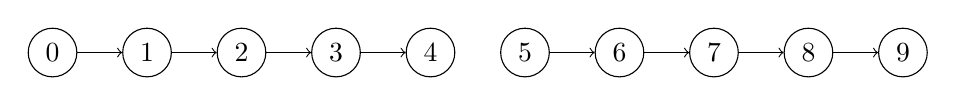
\begin{tikzpicture}
        \foreach \x in {0,1,...,8} {
          \node[circle, draw] (\x) at (1.2*\x,0) {\x};
          }
          \node[circle, draw] (9) at (1.2*9,0) {$9$};
          \foreach[evaluate=\x as \y using int(\x+1.2)] \x in {0,1,...,3} {
            \draw[->] (\x) -- (\y);
            % \draw[->] (\x) to[out=45,in=135] (\x+2);
            % \draw[->] (\x) to[out=60,in=120] (\x+5);
            }
            \foreach[evaluate=\x as \y using int(\x+1.2)] \x in {5,...,8} {
              \draw[->] (\x) -- (\y);
              % \draw[->] (\x) to[out=45,in=135] (\x+2);
              % \draw[->] (\x) to[out=60,in=120] (\x+5);
              }
          \end{tikzpicture}
        \end{center}
      \sol{
        \begin{fig}[label]
          \centering
          
\includegraphics[width=0.5\columnwidth]{\pathtoexos/Info/Figures/graphe_jeu_argent.pdf}
          %\capt{}
        \end{fig}
      }
    \item Définir l'origine $s_0$ du graphe et l'ensemble des sommets finaux $F$ et les colorer sur le graphe précédent. Définir l'ensemble des sommets $S$ et l'ensemble des arcs $A$. Ce graphe $G$ est-il biparti ?
    \sol{
      L’origine est \fbox{$s_0 = 0$}. 
      
      
      L’ensemble des sommets finaux est \fbox{$F = \{4,9\}$}. 
      
      
      L’ensemble des sommets est \fbox{$S = \{0,1,2,3,4,5,6,7,8,9\}$}. 
      
      
      L’ensemble des arcs est 
      \eqbox{
        \begin{split}
          A = \{(0,1),(0,2),(0,5),(1,2),(1,3),(1,6),(2,3),(2,4),(2,7),(3,4),(3,5),(3,8),(5,6),(5,7),\\(6,7),(6,8),(7,8),(7,9),(8,9)\}.
        \end{split}
      }
      
      
      Le graphe $G$ n’est \fbox{pas biparti} car il existe des cycles (non orientés) impairs, par exemple le cycle $ 0 \rightarrow 1 \rightarrow 2 \leftarrow 0$, ce qui interdit d’avoir une bipartition $S  = S_1 \cup S_2$ tels que les arcs relient uniquement les sommets de $S_1$ avec ceux de $S_2$. 
    }
    \item	Implémenter le graphe $G$ dans le langage \texttt{python} sous forme d'une liste d'adjacence, représentée par un dictionnaire \texttt{G}. On rappelle la syntaxe d'un dictionnaire : \texttt{\{clé1:valeur1,clé2:valeur2,...\}}
    \sol{
      {\rm
      \boxed{
    \texttt{G = \{0:[1,2,5],1:[2,3,6],2:[3,4,7],3:[4,5,8],4:[],5:[6,7],6:[7,8],7:[8,9],8:[9],9:[]\}}
      }
      }
    }
    \item Quelle propriété possède l’origine $s_0$ vis-a-vis du dictionnaire \texttt{G} ? Compléter les parties pontillés du code suivant pour définir la fonction \texttt{origine} qui prend en argument le dictionnaire \texttt{G} et renvoie l’origine du graphe. On pourra utiliser la méthode \texttt{liste.remove(element)} qui retire \texttt{element} de \texttt{liste}. Commenter toutes les lignes du code. \emph{Attention : la commande \texttt{liste.remove(element)} renvoie une erreur si \texttt{element} n'est pas dans \texttt{liste} !}
    \inputminted[linenos=true,frame=single]{python}{\pathtoexos/Info/Scripts/origine_G.py}
    \sol{
    L’origine est sans prédécesseurs, donc $\forall s \in S, s_0 \notin G[s]$. On en déduit la fonction \texttt{python} suivante.
    {\rm 
    \inputminted[linenos=true,frame=single]{python}{\pathtoexos/Info/Scripts/origine_G_bis_sol.py}
    }
    }
    \item Effectuer l'exécution pas-à-pas de l'appel \texttt{origine(G)} sur le dictionnaire \texttt{G} défini précédemment, en indiquant la valeur initiale de la liste \texttt{S}, puis la valeur des variables \texttt{s}, \texttt{G[s]}, et \texttt{S} à l'issue de chaque itération dans la boucle, et enfin la valeur de \texttt{S[0]} retournée par la fonction.
    \sol{
      La valeur initiale de \texttt{S} est \texttt{[0,1,2,3,4,5,6,7,8,9]}. 
       \begin{center}
        \begin{tabular}{|c|c|c|c|}
          \hline
          \texttt{s} & \texttt{G[s]} & \texttt{S}(avant) & \texttt{S}(après) \\
          \hline
          \texttt{0} & \texttt{[1,2,5]} & \texttt{[0,1,2,3,4,5,6,7,8,9]} & \texttt{[0,3,4,6,7,8,9]} \\
          \texttt{1} & \texttt{[2,3,6]} & \texttt{[0,3,4,6,7,8,9]} & \texttt{[0,4,7,8,9]} \\
          \texttt{2} & \texttt{[3,4,7]} & \texttt{[0,4,7,8,9]} & \texttt{[0,8,9]} \\
          \texttt{3} & \texttt{[4,5,8]} & \texttt{[0,8,9]} & \texttt{[0,9]} \\
          \texttt{4} & \texttt{[]} & \texttt{[0,9]} & \texttt{[0,9]} \\
          \texttt{5} & \texttt{[6,7]} & \texttt{[0,9]} & \texttt{[0,9]}\\
          \texttt{6} & \texttt{[7,8]} & \texttt{[0,9]} & \texttt{[0,9]} \\
          \texttt{7} & \texttt{[8,9]} & \texttt{[0,9]} & \texttt{[0]} \\
          \texttt{8} & \texttt{[9]} & \texttt{[0]} & \texttt{[0]} \\
          \texttt{9} & \texttt{[]} & \texttt{[0]} & \texttt{[0]} \\
          \hline
        \end{tabular}
       \end{center}
       La fonction renvoie alors 
       \eqbox{
          \texttt{S[0]} = \texttt{0}
       }
      %  \begin{remarque}
        
      %  \end{remarque}
      
    }
    \item Quelle propriété possède les sommets finaux vis-a-vis du dictionnaire \texttt{G} ? Implémenter une fonction \texttt{final} qui prend en argument le dictionnaire \texttt{G} et renvoie la liste \texttt{F} des sommets finaux. Les spécifications de la fonction seront donnés et le code sera commenté.
    \sol{
      {\rm 
    Les sommets finaux sont sans successeurs, soit $G[s] = [~], \forall s \in F$. On en déduit la fonction \texttt{python} suivante.
    \inputminted[linenos=true,frame=single]{python}{\pathtoexos/Info/Scripts/final_G.py}
      }
    }
  \end{quest}
  \parag{Proposition de stratégies}
  Dans la suite, on ne représentera pas le graphe biparti associé à $G$ mais on gardera à l’esprit qu’un même sommet $0 \leq i \leq 9$ peut représenter deux configurations différentes du jeu suivant que le sommet appartient au premier joueur $J_1$ ou au second joueur $J_2$.
    \begin{quest}
    \item Déterminer quels sommets peuvent appartenir à $J_1$ ou $J_2$ et définir les ensembles correspondant $S_1$ et $S_2$. Attention, certains sommets n’appartiennent qu’à un seul des joueurs, tandis que d’autres peuvent appartenir aux deux joueurs.
    \sol{
      \fbox{$S_1 = \{0,2,3,4,5,6,7,8,9\}$} et \fbox{$S_2 = \{1,2,3,4,5,6,7,8,9\}$}. Le sommet $0$ n’appartient qu’à $J_1$ tandis que $1$ n’appartient qu’à $J_2$.
    
    }
    \item 
    On définit la fonction $f : S_1\setminus F \rightarrow S_2$ telle que $f(0) = 5$, $f(2)=4$, $f(3)=4$, $f(5)=7$, $f(6)=8$, $f(7)=9$, et $f(8)=9$. Cette fonction définit-elle une stratégie ? Si oui, cette stratégie est-elle gagnante pour le joueur $J_1$ ? Justifier.  
    \sol{
      L’ensemble de départ est bien défini sur $S_1/F$ car $1 \notin S_1$ et $F=\{4,9\}$. L’ensemble d’arrivée est bien défini car $\{1,5,4,8,9\} \cap S_2$.


      La fonction $f$ définit bien une \boxed{stratégie} car les paires $(0,1)$, $(2,4)$, $(3,4)$, $(5,7)$, $(6,8)$, $(7,9)$, et $(8,9)$ sont bien des arcs.

      La stratégie $f$ n’est \fbox{pas gagnante} pour le joueur $J_1$. En effet, la partie $0 \xrightarrow{J_1} 5 \xrightarrow{J_2} 6 \xrightarrow{J_1} 8 \xrightarrow{J_2} 9$ est jouée suivant $f$ mais perdante pour $J_1$ car le joueur $J_2$ passe de $6$ au sommet final $9$.
    
    }

    \item 
    On définit la stratégie $g : S_2 \setminus F \mapsto S_1$ telle que $g(1) = 6$, $g(2)=4$, $g(3)=4$, $g(5)=6$, $g(6)=7$, $g(7)=9$, et $g(8)=9$. Montrer que cette stratégie est gagnante pour le second joueur $J_2$.
    \sol{
     La stratégie $g$ est \boxed{gagnante} pour le joueur $J_2$. En effet, toutes les  parties jouées suivant $g$ sont de la forme $0 \xrightarrow{J_1} 1,2,5 \xrightarrow{J_2} 4,6 (\xrightarrow{J_1} 7,8 \xrightarrow{J_2} 9)$ et sont gagnantes pour $J_2$.
    }
  \end{quest}

  
  \parag{Algorithme min-max} Pour déterminer de façon certaine s'il existe ou non une stratégie gagnante pour l'un ou l'autre des joueurs, nous appliquons l'algorithme min-max.
  \begin{quest}
    \item Rappeler le principe de l'algorithme min-max. Rappeler l'avantage de la représentation en arbre par rapport à la représentation en graphe. 
    \sol{
      Voir cours. Un graphe représente toutes les configurations du jeu possibles ; une arbre représente toutes les parties possibles.
    }
    
    \item Représenter l'arbre de décision associé à $G$ en indiquant à quel joueur appartiennent les sommets de chaque étage de l'arbre, puis appliquer l'algorithme min-max à la main sur l'arbre de décision. En déduire s'il existe une stratégie gagnante pour $J_1$ ou pour $J_2$.
    \item On implémente la fonction \texttt{minmax} suivante. Compléter les parties pointillées du code en utilisant les méthodes \texttt{max} et \texttt{min} de python, et commenter chaque ligne du code. 
    \inputminted[linenos=true,frame=single]{python}{\pathtoexos/Info/Scripts/minmax_nim.py}
    \sol{
      {\rm
      \inputminted[linenos=true,frame=single]{python}{\pathtoexos/Info/Scripts/minmax_nim_sol.py}
      }}
    \end{quest}


  \parag{Algorithme du noyau} On souhaite vérifier la conclusion précédente par un l'algorithme du noyau. Le \emph{noyau} d'un graphe orienté $G$ est le sous-ensemble de sommets $N \subset S$ tel que :
  \begin{enumerate}[label=(\roman*)]
    \item aucun arc ne joint deux sommets de $N$ :  $\forall s_1,s_2 \in N, (s_1,s_2) \notin A$,
    \item tout sommet hors de $N$ a au moins un successeur dans $N$ : $\forall s_1 \in S \setminus N, \exists s_2 \in N, (s_1,s_2) \in A$. 
  \end{enumerate}
   \begin{quest}
    \item On peut construire le noyau récursivement. Soit $G$ un graphe dont l'ensemble des sommets finaux est $F$. On initialise le noyau par l'ensemble vide puis on procède de la manière suivante :
     \begin{enumerate}
      \item on choisit un sommet final $s \in F$, que l'on ajoute au noyau $N$ ;
      \item on retire de $G$ tous les prédécesseurs $p$ de $s$, ainsi que tous les arcs dont $p$ ou $s$ est une extrémité ;
      \item on répète le processus sur le sous-graphe obtenu jusqu'à ce que le sous-graphe soit vide.
    \end{enumerate}
    Appliquer cet algorithme sur le graphe $G$ précédent à partir du sommet final $s=9$ en représentant à chaque étape le sous-graphe obtenu et le contenu du noyau. Montrer que le noyau du graphe $G$ est l'ensemble $N = \{0,4,6,9\}$.

    \sol{
      Lors de la deuxième étape, le sous-graphe contient deux sommets finaux : 4 et 6. On peut choisir l’un et l’autre de ces sommets pour continuer la procédure.
      \begin{fig}[label]
        \centering
        
\includegraphics[width=0.7\columnwidth]{\pathtoexos/Info/Figures/noyau_G.pdf}
        %\capt{}
      \end{fig}
    }
      \bonus{
    \item On se propose d'implémenter l’algorithme du noyau en deux étapes. Pour commencer, on souhaite définir une fonction \texttt{retrait} qui retire une liste de sommets \texttt{L} d’un graphe \texttt{G}, en mettant à jour les listes d’adjacence.
    Compléter les parties pointillées du code suivant en utilisant la méthode \texttt{remove} de python et commenter chaque nouvelle ligne du code.
      \inputminted[linenos=true]{python}{\pathtoexos/Info/Scripts/noyau_retrait.py}
      \sol{
        \inputminted[linenos=true]{python}{\pathtoexos/Info/Scripts/noyau_retrait_sol.py}
        Veiller à bien mettre la condition \texttt{if s in G[p]} pour éviter que le code ne renvoie une erreur si $s$ n’est pas dans la liste des successeurs de $p$. La méthode \texttt{remove} s’applique à un dictionnaire comme à un graphe.
      }
      \item On propose maintenant de définir une fonction récursive \texttt{noyau} à partir du pseudo-code suivant.
         \begin{center}
      $
      \begin{array}{l}
        \textbf{Si }  G \text{ dictionnaire vide }  \\
           ~~~~|~~ \textbf{Retourner } N  \\  
        f  \leftarrow \text{sommet final } \\
        L \leftarrow \text{liste } [f]  \\
        \textbf{Pour }  s  \text{ dans }G   \\ 
        ~~~~|~~  \textbf{Si }  f \text{ successeur de s} \\
        ~~~~|~~~~|~~  \textbf{Ajouter } s \text{ à } L  \\
        \text{retrait}(G,L)   \\
        \text{noyau}(G,N + [f])   \\
      \end{array}
      $
    \end{center}
    Implémenter la fonction \texttt{noyau(G,N)} en python en précisant les spécifications et en commentant le code. On pourra se servir de la fonction \texttt{final} définie précédemment. Effectuer l’exécution pas à pas de l’appel \texttt{noyau(G,[])} et comparer aux résultats précédents.

    \sol{
      \inputminted[linenos=true,frame=single]{python}{\pathtoexos/Info/Scripts/noyau_jeu_argent.py}
    }
      }
    \item On admet que le noyau $N$ contient l'ensemble des \emph{positions perdantes pour $J_1$}. Le complémentaire du noyau dans $S$ donne au contraire les \emph{positions gagnantes pour $J_1$}. Conclure sur l’existence d’une stratégie gagnante pour $J_1$ ou $J_2$.
    \sol{
    Il existe une stratégie gagnante pour $J_2$ mais pas pour $J_1$.
    }
    \bonus{
    \item Quel autre objet de la théorie des graphes similaire au noyau connaissez-vous qui permette également de trouver les positions gagnantes ? Rappeler sa définition générale sans chercher à déterminer cet objet dans cet exemple précis.
    \sol{
    L’attracteur, voir cours.
    }
    }
  \end{quest}

\end{exo}
%%%%%%%%%%%%%%%%%%%%%%%%%%%%%%%%%%%


%%%%%%%%%%%%%%%%%%%%%%%%%%%%%%%%%%%
\begin{exo}[PC][1][devoir]{Nombre de Grundy}
  
On considère un jeu de Nim avec un tas où chaque joueur peut retirer de $1$ à $p$ objets. Celui que ne peut plus retirer d'objets a perdu. Une position est déterminée par le nombre $n$ d'objets présents dans le tas.
À chaque position $n$, on associe le nombre noté $g(n)$, appelé nombre de Grundy, défini récursivement par :
\begin{liste}
  \item le nombre de Grundy de la position finale vaut $0$, soit $g(0)=0$ ;
  \item le nombre de Grundy d'une position $n$ est le plus petit entier naturel qui n'est pas le nombre de Grundy d'une des positions directement atteignables depuis la position $n$.
\end{liste}

On commence par étudier le jeu de Nim pour $p=2$.
\emph{Par exemple, depuis la position $n=4$ on peut atteindre les positions $3$ et $2$. Si $g(3)=0$ et $g(2)=2$, alors $g(4)=1$.}

\begin{quest}
  %\item Le nombre de Grundy correspond-il à la définition d'une heuristique ? Justifier.
    \item Montrer par récurrence sur $n$ que $g(n)=r$ où $r$ est le reste de la division euclidienne de $n$ par~$3$, soit $n=3q+r$.
    \sol{
    \begin{liste}
      \item $\underline{n=0}$. Par définition, $g(0)=0$. Pour l’exemple, on peut aussi vérifier que $g(1)=1$, car la position $0$ est le seul successeur de $1$. De même, $g(2)=2$, car les successeurs de $2$ sont $0$ et $1$, de nombres de Grundy $0$ et $1$.
       %Soit une position $r$ tell que $0\leq r \leq p$. On montre que $g(r) = r$.
        %Depuis la position $0 \leq r \leq p$, un joueur peut atteindre toutes les positions de $0$ à $r-1$, et donc $g(r)=r$.
        \item Supposons la propriété vraie pour toutes \underline{positions $\leq n$}.

        Depuis la position $n+1=3q+r$ avec $0 \leq r \leq 2$ et $q\geq1$, un joueur peut atteindre les positions $n-1$ et $n-2$. Si $r=0$, alors $n-1=3(q-1)+2$ et $n-2=3(q-1)+1$, de nombres de Grundy $g(n-1)=2$ et $g(n-2)=1$. Donc $g(n) = 0 =r$.  Si $r=1$, alors $n-1=3q$ et $n-2=3(q-1)+2$,
        de nombres de Grundy $g(n-1)=0$ et $g(n-2)=2$. Donc $g(n) = 1 =r$.  Si $r=2$, alors $n-1=3q+1$ et $n-2=3q$, de nombres de Grundy $g(n-1)=1$ et $g(n-2)=0$. Donc $g(n) = 2 =r$. La relation est donc vérifiée pour $n+1$.
    \end{liste}
    }
\end{quest}
On admet que ce résultat se généralise à $p$ quelconque : pour tout entier naturel $n$, le nombre de Grundy vaut $g(n)=r$ où $r$ est le reste de la division euclidienne de $n$ par $p+1$.
  % On pourra raisonner par récurrence sur le quotient $q$ de la division euclidienne $n=q(p+1)+r$.
\begin{quest}
  \item Le théorème de Sprague-Grundy, établi dans les années 1930, affirme qu'une position dont le nombre de Grundy vaut $0$ est une position gagnante à atteindre. En déduire une stratégie gagnante $f$ pour $J_1$ suivant la valeur de $n$. Existe-t-elle toujours ?
  \sol{
  Le joueur doit atteindre une position qui est un multiple de $p+1$. En effet, $g((p+1)q)=0$. On peut donc choisir comme stratégie $f: n=(p+1)q+r \mapsto (p+1)q$ si $1\leq r \leq 2$. Par contre, si $n \in J_1$ est un multiple de $p+1$, il n’existe pas de stratégie gagnante.
  }
  \item Représenter le graphe du jeu $G$ pour $n=5$ et $p=2$.
  \sol{
  \begin{fig}[]
    \centering
    
\includegraphics[width=0.3\textwidth]{Grundy_jeu.png}
    
\includegraphics[width=0.5\textwidth]{Grundy_biparti_jeu.png}
    \capt{}
  \end{fig}
  }
  %, où chaque sommet correspond à une position $n$.
  Comment rendre simplement ce graphe biparti ? Représenter alors l'arène $(G,S_1,S_2)$ en dessinant les sommets appartenant à $J_1$ et $J_2$ d'une couleur différente. Indiquer les sommets initiaux et finaux.
  \item Définir le graphe précédent sous \texttt{python} sous forme de dictionnaire. Une clé est un couple $(j,n)$ où $j$ est le numéro du joueur contrôlant le sommet et $n$ est le nombre d'objets restants. Une valeur est une liste de successeurs.
  \sol{
  \inputminted{python}{\pathtoexos/Info/Scripts/G_grundy.py}
  }
  % La position initiale est $(1,n)$. La position finale gagnante à atteindre pour $J_1$ est $(2,0)$.
  \item On souhaite calculer l'attracteur du graphe précédent. Que vaut l'ensemble \texttt{F} des sommets finaux pour $J_1$ ? On donne ci-dessous une fonction définie en \texttt{python} pour calculer l'attracteur d'une graphe $G$ défini sous forme de dictionnaire.
  %\inputminted{python}{/home/eric/Dropbox/CPGE/Physique/Exercices/Recueil/Info/Scripts/attract2_sol.py}
  % \inputminted{python}{/home/eric/Dropbox/CPGE/Physique/Exercices/Recueil/Info/Scripts/attract3_sol.py}
  \inputminted{python}{\pathtoexos/Info/Scripts/attract_ds.py}
  On suppose avoir prédéfini les fonctions \texttt{existe} et \texttt{pourtout} telles que \texttt{existe(G,F,J)}$=\{s \in S_J, \exists \text{ arc } (s,t) \text{ avec } t \in F\}$ et \texttt{pourtout(G,F,J)}$=\{s \in S_J, \forall \text{ arc } (s,t),  t \in F\}$, pour tout joueur $J=1,2$.
  Effectuer une exécution pas à pas de la commande \texttt{attract(G,F)} où $G$ désigne le graphe du jeu pour $n=5$ et $p=2$.
  %On pourra indiquer directement le résultat de la commande \texttt{inverse(G)} sans exécuter la fonction \texttt{inverse} pas à pas.
  Que vaut l'attracteur $A$ ? Comparer à la stratégie gagnante obtenue par le théorème de Sprague-Grundy.
  \sol{
  Le sommet gagant pour $J_1$ (qui appartient à $J_2$) est $(2,0)$. Donc  $F = \{(2,0)\}$.

  Exécution pas à pas de \texttt{attract(G,F)}.
      \underline{Erratum} : pour que la condition du \texttt{if} soit correcte, il faudrait préciser que \texttt{existe} et \texttt{pourtout} renvoie uniquement les éléments qui ne sont pas déjà compris dans $F$. On va supposer que c’est le cas par la suite.
  \begin{liste}
    \item $E =$ \texttt{existe(G,F,1)} $= [(1,1),(1,2)]$ puisqu’on peut atteindre $0$ à partir de $1$ et $2$.
    \item $P =$ \texttt{pourtout(G,F,2)} $= []$
    est vide puisque $(2,0) \in J_2$.
    \item $A = [(2,0),(1,1),(1,2)]$.
    \item $E \neq []$ donc on renvoie \texttt{attract(G,[(2,0),(1,1),(1,2)])}.
    \begin{liste}
      \item Ici $E = []$, tandis que $P = [(2,3)]$.
      \item $A = [(2,0),(1,1),(1,2),(2,3)]$.
      \item $P \neq []$ donc on renvoie \texttt{attract(G,[(2,0),(1,1),(1,2),(2,3)])}.
      \begin{liste}
        \item Ici $E = [(1,4),(1,5)]$, et $P = []$.
        \item $A = [(2,0),(1,1),(1,2),(2,3),(1,4),(1,5)]$
        \item $E \neq []$ donc on renvoie \texttt{attract(G,[(2,0),(1,1),(1,2),(2,3),(1,4),(1,5)])}.
        \begin{liste}
          \item Ici $E = []$ et $P = []$, donc la condition \texttt{if} est vérifiée et on retourne $A = [(2,0),(1,1),(1,2),(2,3),(1,4),(1,5)]$
        \end{liste}
      \end{liste}
    \end{liste}
  \end{liste}
  Une fois toute la chaîne remontée, le programme retourne l’attracteur
  $$
  A = [(2,0),(1,1),(1,2),(2,3),(1,4),(1,5)].
  $$
  Comme l’origine $(1,5) \in A$ appartient à l’attracteur, il existe une stratégie gagnante. Celle-ci, notée $f : S_1 \rightarrow S_2$, s’obtient en suivant la liste des sommets ajoutés à $A$ pour construire l’attracteur. Donc $f(1,5) = f(2,3)$, $f(1,1)=(2,0)$ et $f(1,2)=(2,0)$. La valeur de $f(1,4)$ n’est pas importante. Cette stratégie gagnante est cohérente avec celle obtenue par le théorème de Sprague-Grundy.
  }
\end{quest}
\end{exo}
%%%%%%%%%%%%%%%%%%%%%%%%%%%%%%%%%%%

%%%%%%%%%%%%%%%%%%%%%%%%%%%%%%%%%%%
\begin{exo}[PC][1][devoir]{Le jeu du morpion}
  
Le jeu du morpion est un jeu séquentiel à deux joueurs antagonistes, dont le principe est d'aligner plusieurs symboles identiques sur une grille. Dans la version classique du jeu, la grille est de taille $3\times3$. Les joueurs dessinent un symbole sur une case à tour de rôle (une croix pour un joueur, un cercle pour l'autre joueur).
Un joueur gagne s'il atteint une configuration où il a aligné trois symboles horizontalement, verticalement, ou diagonalement.

\begin{fig}
  \centering
  
\includegraphics{\pathtoexos/Info/Figures/tic-tac-toe_0.pdf}
  \capt{Configuration initiale étudiée d'un jeu de morpion sur une grille $3\times 3$. C'est au joueur $J_1$ de jouer à partir de cette configuration initiale. Le joueur $J_1$ trace des croix, tandis que le joueur $J_2$ trace des cercles. }
  \label{fig:morpion}
\end{fig}

\subsection{Modélisation du jeu}

\begin{quest}
  \item Combien y a-t-il de configurations de jeu possibles à partir de la configuration initiale de la \Fig{morpion} ?
  Représenter graphiquement le graphe $G$ associé en représentant les configurations de jeu à chaque sommet. Indiquer à quel joueur, $J_1$ ou $J_2$, appartient chaque sommet, puis identifier les sommets finaux du graphe et indiquer pour chacun qui du joueur $J_1$ ou $J_2$ est gagnant. \emph{Attention, dans ce jeu, un sommet peut appartenir à $J_1$ et être gagnant pour $J_2$, et vice versa.}
\sol{
On peut s’attentre à $3+3\times2+3\times2\times1 = 15$ configurations au total, mais en réalité certaines n’interviennent pas parce qu’un joueur gagne avant. En traçant le graphe, on voit qu’il existe $4$ configurations non atteintes parce que $J_2$ gagne avant, et que $2$ configurations conduisent à $1$ configuration commune, ce qui réduit le nombre de configurations à $10$ (numérotées de $1$ à $10$, sans compter l’origine).
\begin{fig}[]
  \centering
  
\includegraphics[width=0.9\textwidth]{graphe_morpion.png}
  \capt{}
\end{fig}
}
  %. La configuration initiale est notée~$0$.
  %\item Montrer graphiquement que ce graphe est biparti. Identifier les ensembles $S_1$ (sommets appartenant à $J_1$) et $S_2$ (sommets appartenant à $J_2$), ainsi que les ensembles de sommets finaux correspondants $F_1$ et $F_2$.
  %\item
\end{quest}
Dans la suite, on associera un numéro $n$ à chaque configuration de jeu, suivant le \Tab{numerotation_morpion}. On représentera donc chaque sommet du graphe par ce seul numéro.
\begin{table}[H]
  \centering
  \begin{tabular}{|c|c|c|c|c|c|c|c|}
    \hline
    
\includegraphics[scale=0.5]{\pathtoexos/Info/Figures/tic-tac-toe_0.pdf} & 
\includegraphics[scale=0.5]{\pathtoexos/Info/Figures/tic-tac-toe_1.pdf} & 
\includegraphics[scale=0.5]{\pathtoexos/Info/Figures/tic-tac-toe_2.pdf} & 
\includegraphics[scale=0.5]{\pathtoexos/Info/Figures/tic-tac-toe_3.pdf} & 
\includegraphics[scale=0.5]{\pathtoexos/Info/Figures/tic-tac-toe_4.pdf} & 
\includegraphics[scale=0.5]{\pathtoexos/Info/Figures/tic-tac-toe_5.pdf} & 
\includegraphics[scale=0.5]{\pathtoexos/Info/Figures/tic-tac-toe_6.pdf} & 
\includegraphics[scale=0.5]{\pathtoexos/Info/Figures/tic-tac-toe_7.pdf}  \\
    \hline
    0 & 1 & 2 & 3 & 4 & 5 & 6 & 7  \\
    \hline
  \end{tabular}

  \begin{tabular}{|c|c|c|}
  \hline
 
\includegraphics[scale=0.5]{\pathtoexos/Info/Figures/tic-tac-toe_8.pdf} & 
\includegraphics[scale=0.5]{\pathtoexos/Info/Figures/tic-tac-toe_9.pdf} & 
\includegraphics[scale=0.5]{\pathtoexos/Info/Figures/tic-tac-toe_10.pdf} \\
 \hline
 8 & 9 & 10 \\
 \hline
\end{tabular}
  
\caption{Numérotation des configurations de jeu rencontrées dans le jeu du morpion.}
\label{tab:numerotation_morpion}
\end{table}

%, et utiliser ce numéro pour représenter les sommets.
\begin{quest}
  \item Représenter graphiquement l'arbre de décision $A$ associé au graphe $G$.
  %, en représentant les configurations de jeu à chaque nœud.
  Indiquer à quel joueur, $J_1$ ou $J_2$, appartient chaque nœud, puis identifier les feuilles de l'arbre et indiquer pour chacune qui du joueur $J_1$ ou $J_2$ est gagnant.
  \sol{
  \begin{fig}[]
    \centering
    
\includegraphics[width=0.4\textwidth]{Arbre_morpion.png}
    \capt{}
  \end{fig}
  }
\end{quest}

\subsection{Heuristique et algorithme min-max}

On définit une heuristique $h$ pour le joueur $J_1$ sur l'ensemble des nœuds de l’arbre de décision précédent de la façon suivante.
\begin{liste}
  \item À chaque case $c$ de la grille, on associe un entier $a(c)$ correspondant au nombre d'alignements horizontal, vertical, ou diagonal qu'il est possible de réaliser à partir de cette case, en supposant toutes les autres cases vides.

  \emph{Par exemple, cet entier est maximal pour la case centrale, où il vaut 4}.
  \item À chaque nœud $s$ de l'arbre de décision, on définit $h(s)$ par la somme des entiers $a(c)$ pour toutes les cases $c$ occupées, comptés positivement pour les croix et négativement pour les cercles.
\end{liste}

\begin{quest}
  \item Justifier que $h$ correspond bien à la définition d'une heuristique.
  \sol{
  Voir cours : $h$ est d’autant plus grande que la position est avantageuse pour $J_1$, et d’autant plus petit que la position est désavantageuse pour $J_2$.
  }
  \item Représenter la grille de morpion en indiquant dans chaque $c$ la valeur du nombre d'alignements potentiels $a(c)$. En déduire l'heuristique $h(0)$ pour la configuration initiale de la \Fig{morpion}.
  \sol{
  \begin{fig}[]
    \centering
    
\includegraphics[width=0.3\textwidth]{cases_morpion.png}
    \capt{}
  \end{fig}
  L’heuristique de la position initiale vaut $h(0) = (3+2+2)-(3+3+3)=-2$. L’heuristique est négative, ce qui est cohérent avec le caractère plutôt désavantageux de cette configuration ($J_1$ ne possède qu’une configuration gagnante, alors que $J_2$ en possède $4$).
  }
  \item Déterminer et représenter les valeurs de $h(s)$ pour tous les nœuds $s$ du niveau $1$ de l'arbre (les successeurs immédiats de la configuration initiale). Laquelle de ces configurations $J_1$ a-t-il intérêt à choisir ?
  \sol{
  \begin{fig}[]
    \centering
    
\includegraphics[width=0.4\textwidth]{arbre_h1.png}
    \capt{}
  \end{fig}
$J_1$ veut maximiser l’heuristique. Il jouera donc la configuration $2$, d’heuristique $h(2)=2$.
  }
  \item Faire de même pour tous les nœuds du niveau $2$ de l'arbre. En suivant la stratégie qui consiste à maximiser l'heuristique, quel coup le joueur $J_1$ doit-il jouer à partir de la configuration initiale ? Cela lui permet-il de gagner ? Justifier que cette définition de l'heuristique n'est pas un bon choix.
  %  Pourquoi ?
  \sol{
  \begin{fig}[]
    \centering
    
\includegraphics[width=0.4\textwidth]{arbre_h2.png}
    \capt{}
  \end{fig}
Connaissant les valeurs d’heuristique au $2^e$ niveau de l’arbre, $J_1$ jouera encore la configuration $2$, puis l’une au l’autre des configurations $8$ ou $9$, de mêmes heuristique $h(8)=h(9)=0$. Le problème est que $8$ est gagnant pour $J_2$, alors que $9$ permet à $J_1$ de gagner. De plus, la configuration $5$, qui permet ensuite à $J_1$ de gagner, a une heuristique plus faible que $8$, qui est gagnant pour $J_2$ ! $h$ n’est donc pas un bon choix d’heuristique.
  }
\end{quest}

On choisit une autre heuristique $h'$ définie sur l'arbre de décision de la façon suivante.
\begin{liste}
  \item Sur une feuille $f$, l'heuristique vaut $h'(f)=+1$ si la configuration est gagnante pour $J_1$, et $h'(f)=-1$ sinon.
  \item Sur un nœud $s$, l'heuristique $h'(s)$ est déterminée par l'algorithme min-max : si $s \in J_1$, $h'(s)$ est égal au maximum des heuristiques des successeurs de $s$ ; si  $s \in J_2$, $h'(s)$ est égal au minimum des heuristiques des successeurs de $s$.
\end{liste}

\begin{quest}
  \item Représenter l'arbre de décision en indiquant à côté de chaque nœud $s$ la valeur de $h'(s)$. Existe-t-il une stratégie gagnante pour $J_1$ ?
  \sol{
  \begin{fig}[]
    \centering
    
\includegraphics[width=0.6\textwidth]{hp_jeu.png}
    \capt{}
  \end{fig}
  Comme $h(0)=-1$, il n’existe pas de stratégie gagnante pour $J_1$.
  }
  \item On représente l'arbre de décision $A$ par un dictionnaire dont chaque clé $s=(j,n)$ représente un nœud de numéro $n$ et appartenant au joueur $j=1,2$, et chaque valeur représente la liste des nœuds successeurs. Définir \texttt{A} en \texttt{python}.
  \sol{
  \inputminted{python}{\pathtoexos/Info/Scripts/A_arbre.py}
  }
  \item On définit ci-dessous la fonction \texttt{minmax} qui applique l'algorithme min-max pour calculer l'heuristique d'un nœud $s$.
    \inputminted{python}{\pathtoexos/Info/Scripts/minmax.py}
  Compléter et commenter chaque ligne de ce code. On pourra utiliser les fonctions \texttt{min} et \texttt{max}. Exécuter pas à pas la commande \texttt{minmax(A,(1,0))} où \texttt{A} est l'arbre de décision défini précédemment. Comparer au résultat de la question précédente.
  \sol{
  \inputminted{python}{\pathtoexos/Info/Scripts/minmax_sol.py}
  \begin{liste}
    \item Exécution de \texttt{minmax(A,(1,0))}.\\
      $A[(1,0)] \neq []$ puis $h_0=[\texttt{minmax(A,(2,1))},\texttt{minmax(A,(2,2))},\texttt{minmax(A,(2,3))}]$.
      \begin{liste}
        \item  Exécution de \texttt{minmax(A,(2,1))}.\\
        $A[(2,1)] \neq []$ puis $h_1=[\texttt{minmax(A,(1,6))},\texttt{minmax(A,(1,7))]}$.
        \begin{liste}
        \item  Exécution de \texttt{minmax(A,(1,6))}.\\
        $A[(1,6)] = []$ puis $(1,6)[0]=1$ donc renvoie $-1$.
        \item  Idem pour \texttt{minmax(A,(1,7))} : renvoie $-1$.
        \end{liste}
        \item On remonte la chaîne d’exécution à \texttt{minmax(A,(2,1))} : $h_1=[-1,-1]$ puis $(2,1)[0]=2$ donc renvoie $\text{min}(h_1)=-1$.
        \item Idem pour \texttt{minmax(A,(2,2))} et pour \texttt{minmax(A,(2,3))} : renvoie $-1$.
      \end{liste}
      \item On remonte la chaîne d’exécution à \texttt{minmax(A,(1,0))} : $h_0=[-1,-1,-1]$ puis $(1,0)[0]=1$ donc renvoie $\text{max}(h_0)=-1$.
  \end{liste}
  }
\end{quest}

% \subsection{Algorithme de l'attracteur}

% On souhaite déterminer l'attracteur du graphe $G$ associé au jeu du morpion. On définit l'attracteur d'un graphe orienté $G$ de la façon récursive suivante.
% \begin{liste}
%   \item On initialise l'attracteur $A$ à l'ensemble vide.
%   \item On détermine l'ensemble $E$ des sommets $s$ tels qu'il existe un arc $(s,t)$ avec $t \in A$.
%   \item On détermine l'ensemble $P$ des sommets $s$ tels que pour tout arc $(s,t)$, $t \in A$.
%   \item Si $E$ ou $P$ sont non vide, on ajoute $E$ et $P$ à l'attracteur $A$.
%   \item Sinon, on renvoie l'attracteur $A$.
% \end{liste}
% \begin{quest}
%   \item	Appliquer l'algorithme de l'attracteur au graphe $G$ associé au jeu du morpion représenté précédemment.
% \end{quest}


\end{exo}
%%%%%%%%%%%%%%%%%%%%%%%%%%%%%%%%%%%